\section{Trasowanie Cebulowe}

\sebsection{Ogólna zasada działania}
Zasada działania sieci Tor opiera się na rozproszonej grupie węzłów pośredniczących, administrowanych przez ochotników. Takie urządzenia nazywane są Routerami Cebulowymi (ang. Onion Routers). 

Ogólna zasada działania sieci Tor wygląda następująco:
\begin{enumerate}
  \begin{figure}
    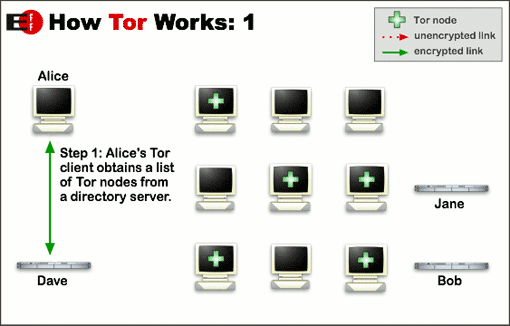
\includegraphics[width=\textwidth]{dzialanie_tor_1}
  \end{figure}
  \item Na początku oprogramowanie klienckie, nazywane Cebulowym Proxy, pobiera listę wszystkich działających Routerów Cebulowych, wraz z~ich kluczami publicznymi, następnie zostaje wybranych kilku spośród nich, które będą tworzyć obwód (ang. circuit) pomiędzy klientem, a~serwerem docelowym. 
  \begin{figure}
    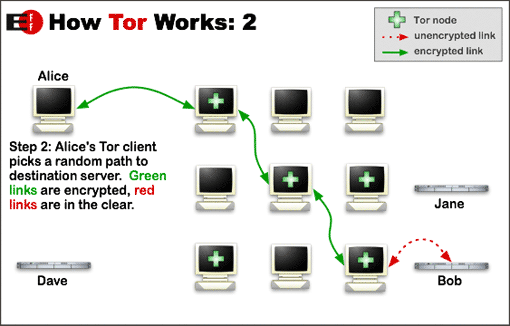
\includegraphics[width=\textwidth]{dzialanie_tor_2}
  \end{figure} 
  \item W kolejnym kroku zostaje stworzony obwód z~wybranych wcześniej węzłów pośredniczących.
  \item Następnie klient wielokrotnie szyfruje przesyłaną wiadomość, gdzie każda warstwa szyfru jest tworzona za pomocą publicznych kluczy cebulowych Routerów Cebulowych w~odwrotnej kolejności niż znajdują się one we wcześniej utworzonym obwodzie (ostatnia warstwa szyfru jest stworzona za pomocą publicznego klucza Routera Cebulowego znajdującego się na początku obwodu, a~ta znajdująca się najgłębiej, za pomocą klucza publicznego ostatniego Routera Cebulowego, znajdującego się w~obwodzie).
  \begin{figure}
    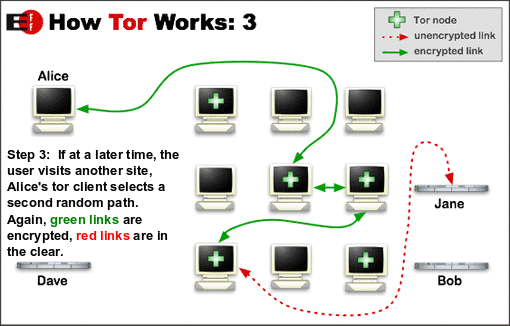
\includegraphics[width=\textwidth]{dzialanie_tor_3}
  \end{figure}
  \item W~kolejnym kroku zaszyfrowana wiadomość zostaje przesłana do pierwszego węzła w~obwodzie. W~tej postaci znany jest tylko adres klienta, oraz pierwszego węzła, do którego ma trafić. 
  \item Serwer, który ją odebrał odszyfrowuje ją za pomocą swojego klucza prywatnego, co powoduje odkrycie adresu następnego Routera Cebulowego do którego wiadomość ma zostać przekazana.
  \item Następnie wiadomość ta zostaje przesłana do kolejnego węzła.
  \item Proces ten jest kontynuowany do momentu, w którym wiadomość trafia do ostatniego węzła w~obwodzie, który to zdejmuje ostatnią warstwę szyfru. \item Niezaszyfrowana wiadomość zostaje przesłana do docelowego serwera.
\end{enumerate}

